\clearpage
\begin{appendices}

\chapter{Evaluation of Pruning for Model Lightweighting}
\label{app:pruning}

This appendix reports the pruning experiments conducted on the MIT-BIH
Arrhythmia Database and clarifies the rationale for adopting Depthwise
Separable Convolution (DSConv) for the final mobile deployment.
Classes follow AAMI EC57: N (normal and bundle-branch block), S
(supraventricular ectopic), V (ventricular ectopic), and F (fusion).
These experiments use models trained on MIT-BIH with the AAMI EC57 label
set, which differs from the HiCardi multi-label setting used elsewhere in
this thesis; the latencies reported below are therefore not directly
comparable to the HiCardi-trained, final-deployment-graph latencies in
Table~\ref{tab:delegation_scope}.

\begin{figure}[h]
  \centering
  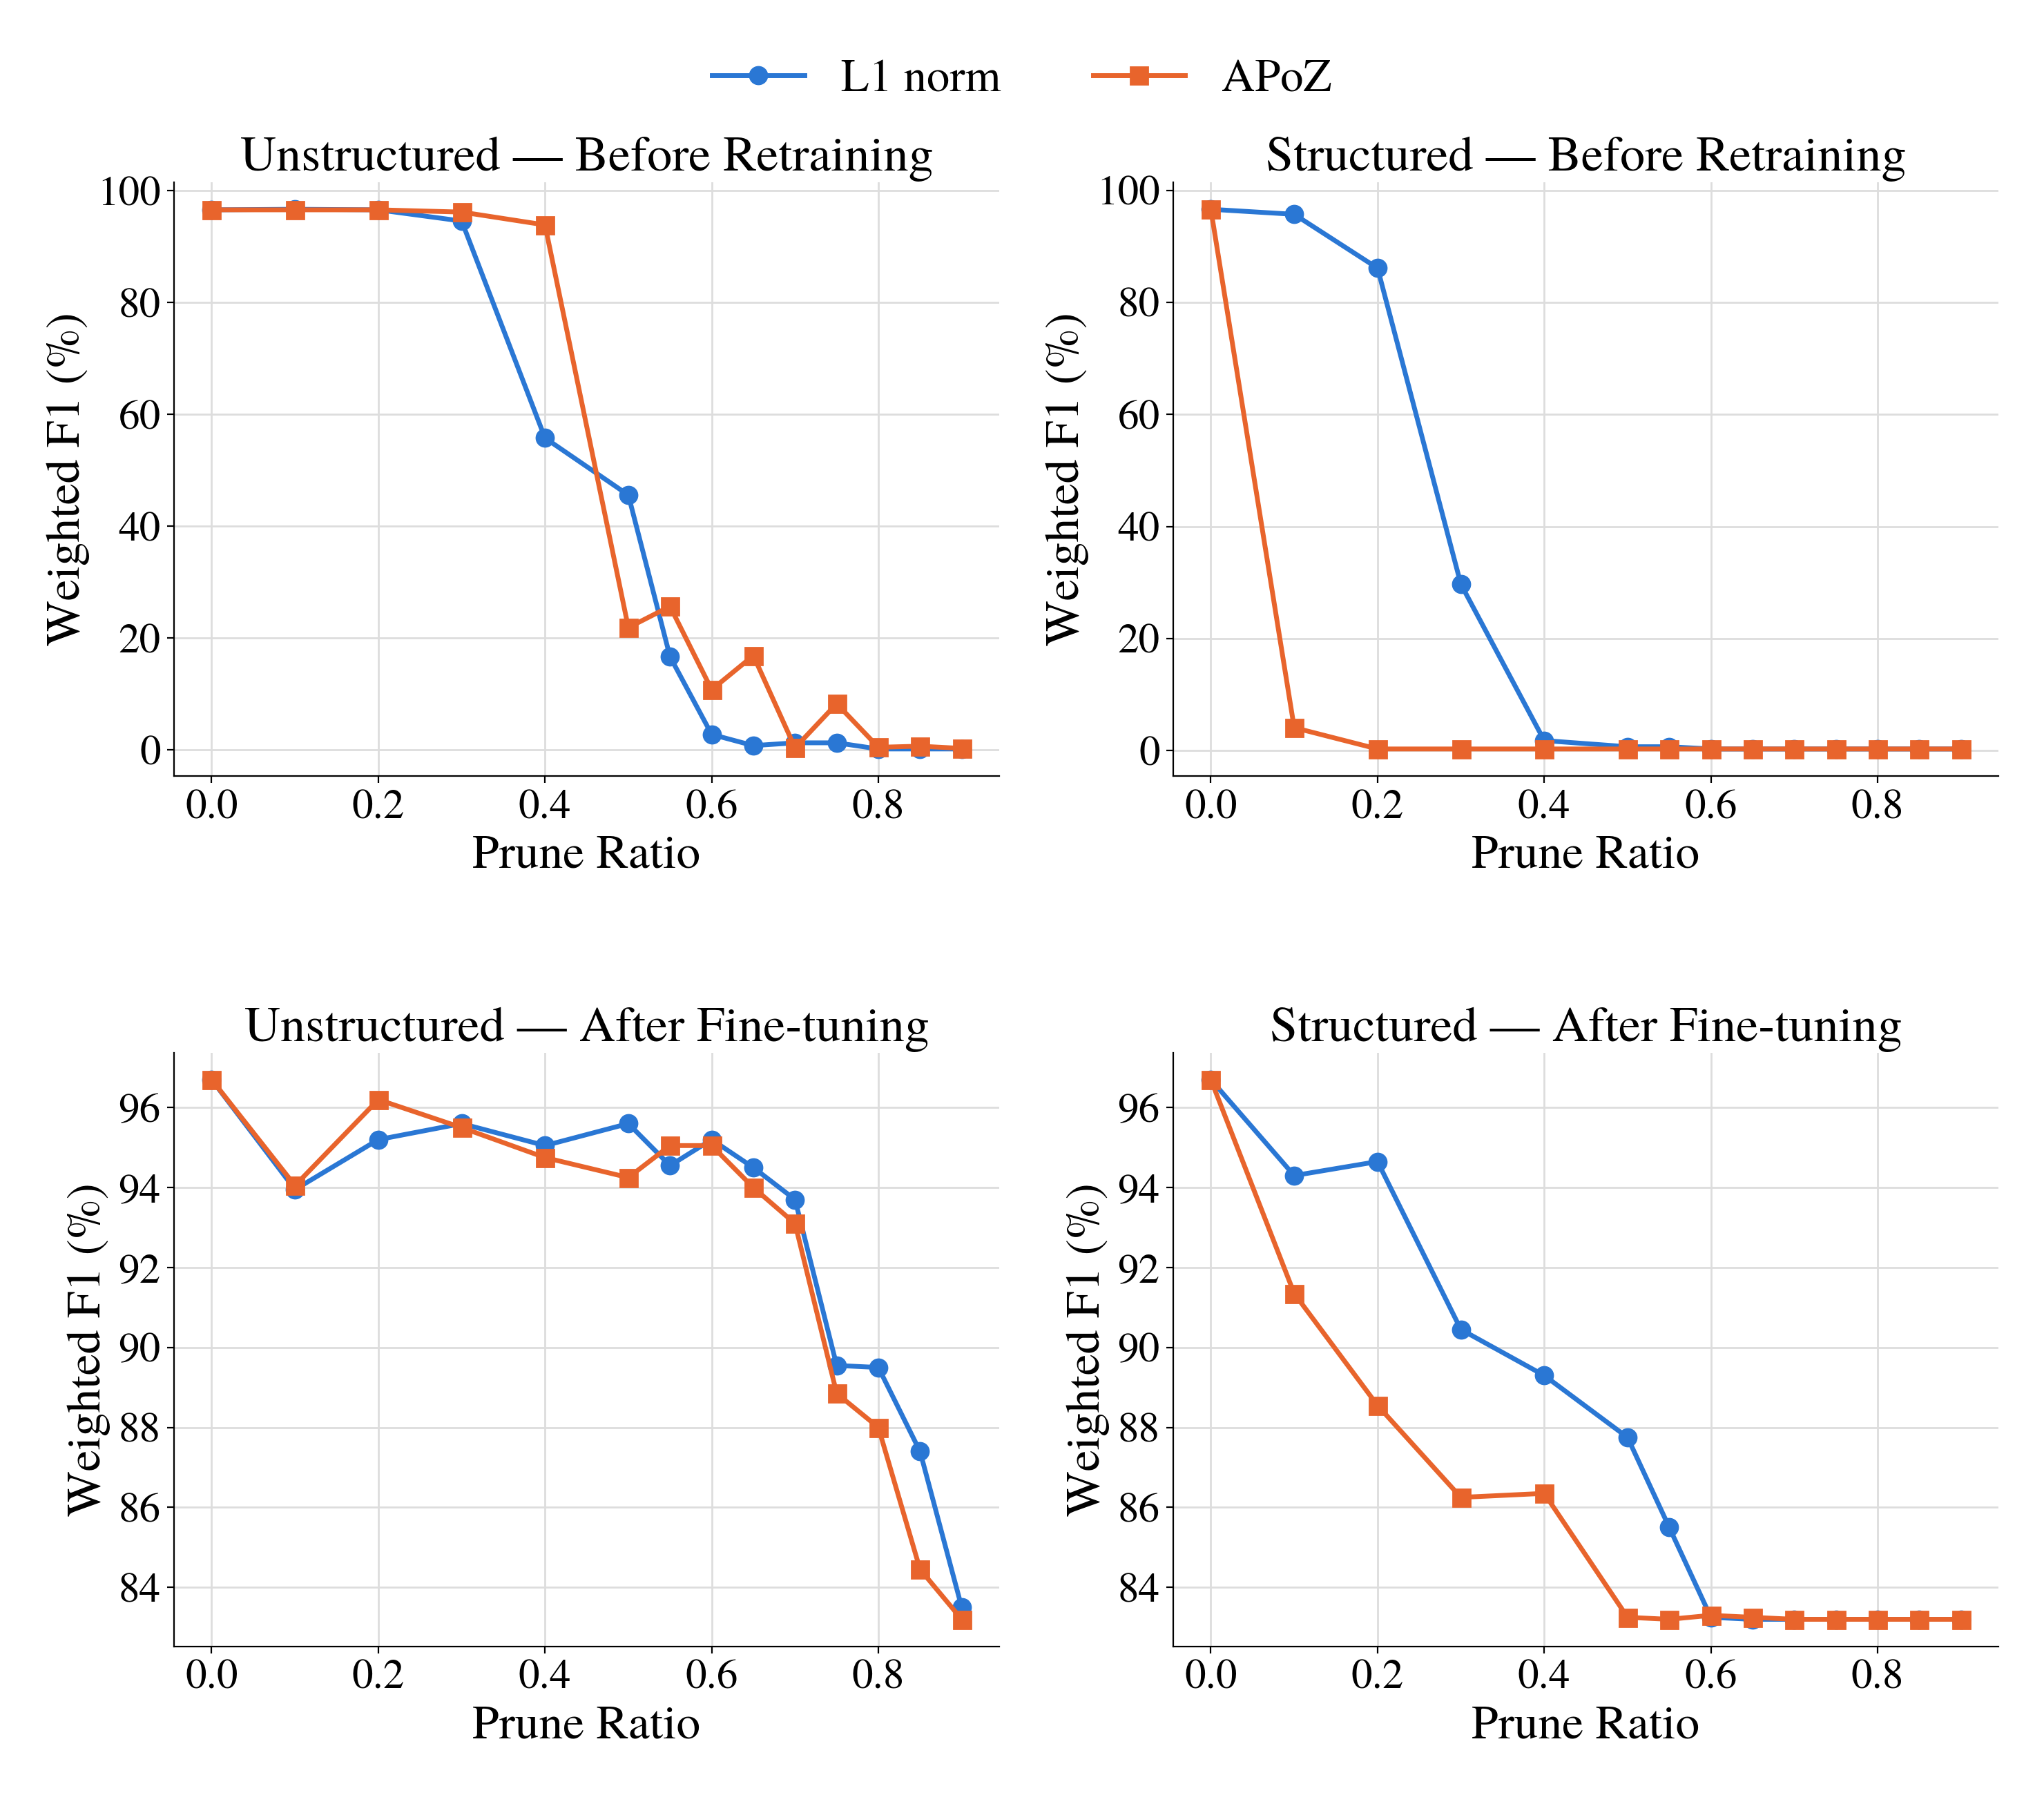
\includegraphics[width=\textwidth]{figures/fig_pruning.png}
  \caption[Weighted $F_1$ versus prune ratio.]{Weighted $F_1$ versus
  prune ratio on MIT-BIH. Left: unstructured pruning; right: structured
  pruning. Top: before retraining; bottom: after fine-tuning.}
  \label{fig:app_pruning_f1}
\end{figure}

Pruning was initially evaluated as an alternative method to reduce the
model size. Fig.~\ref{fig:app_pruning_f1} shows the effect of
unstructured (left) and structured (right) pruning on classification
performance. After fine-tuning (bottom row), unstructured pruning
maintains the weighted $F_1$ score up to a ratio of 0.7. However,
structured pruning degrades sharply from the first non-zero ratio,
settling near a trivial majority-class baseline (labeling every beat N
yields an $F_1$ of $82.1\,\%$).

\begin{figure}[h]
  \centering
  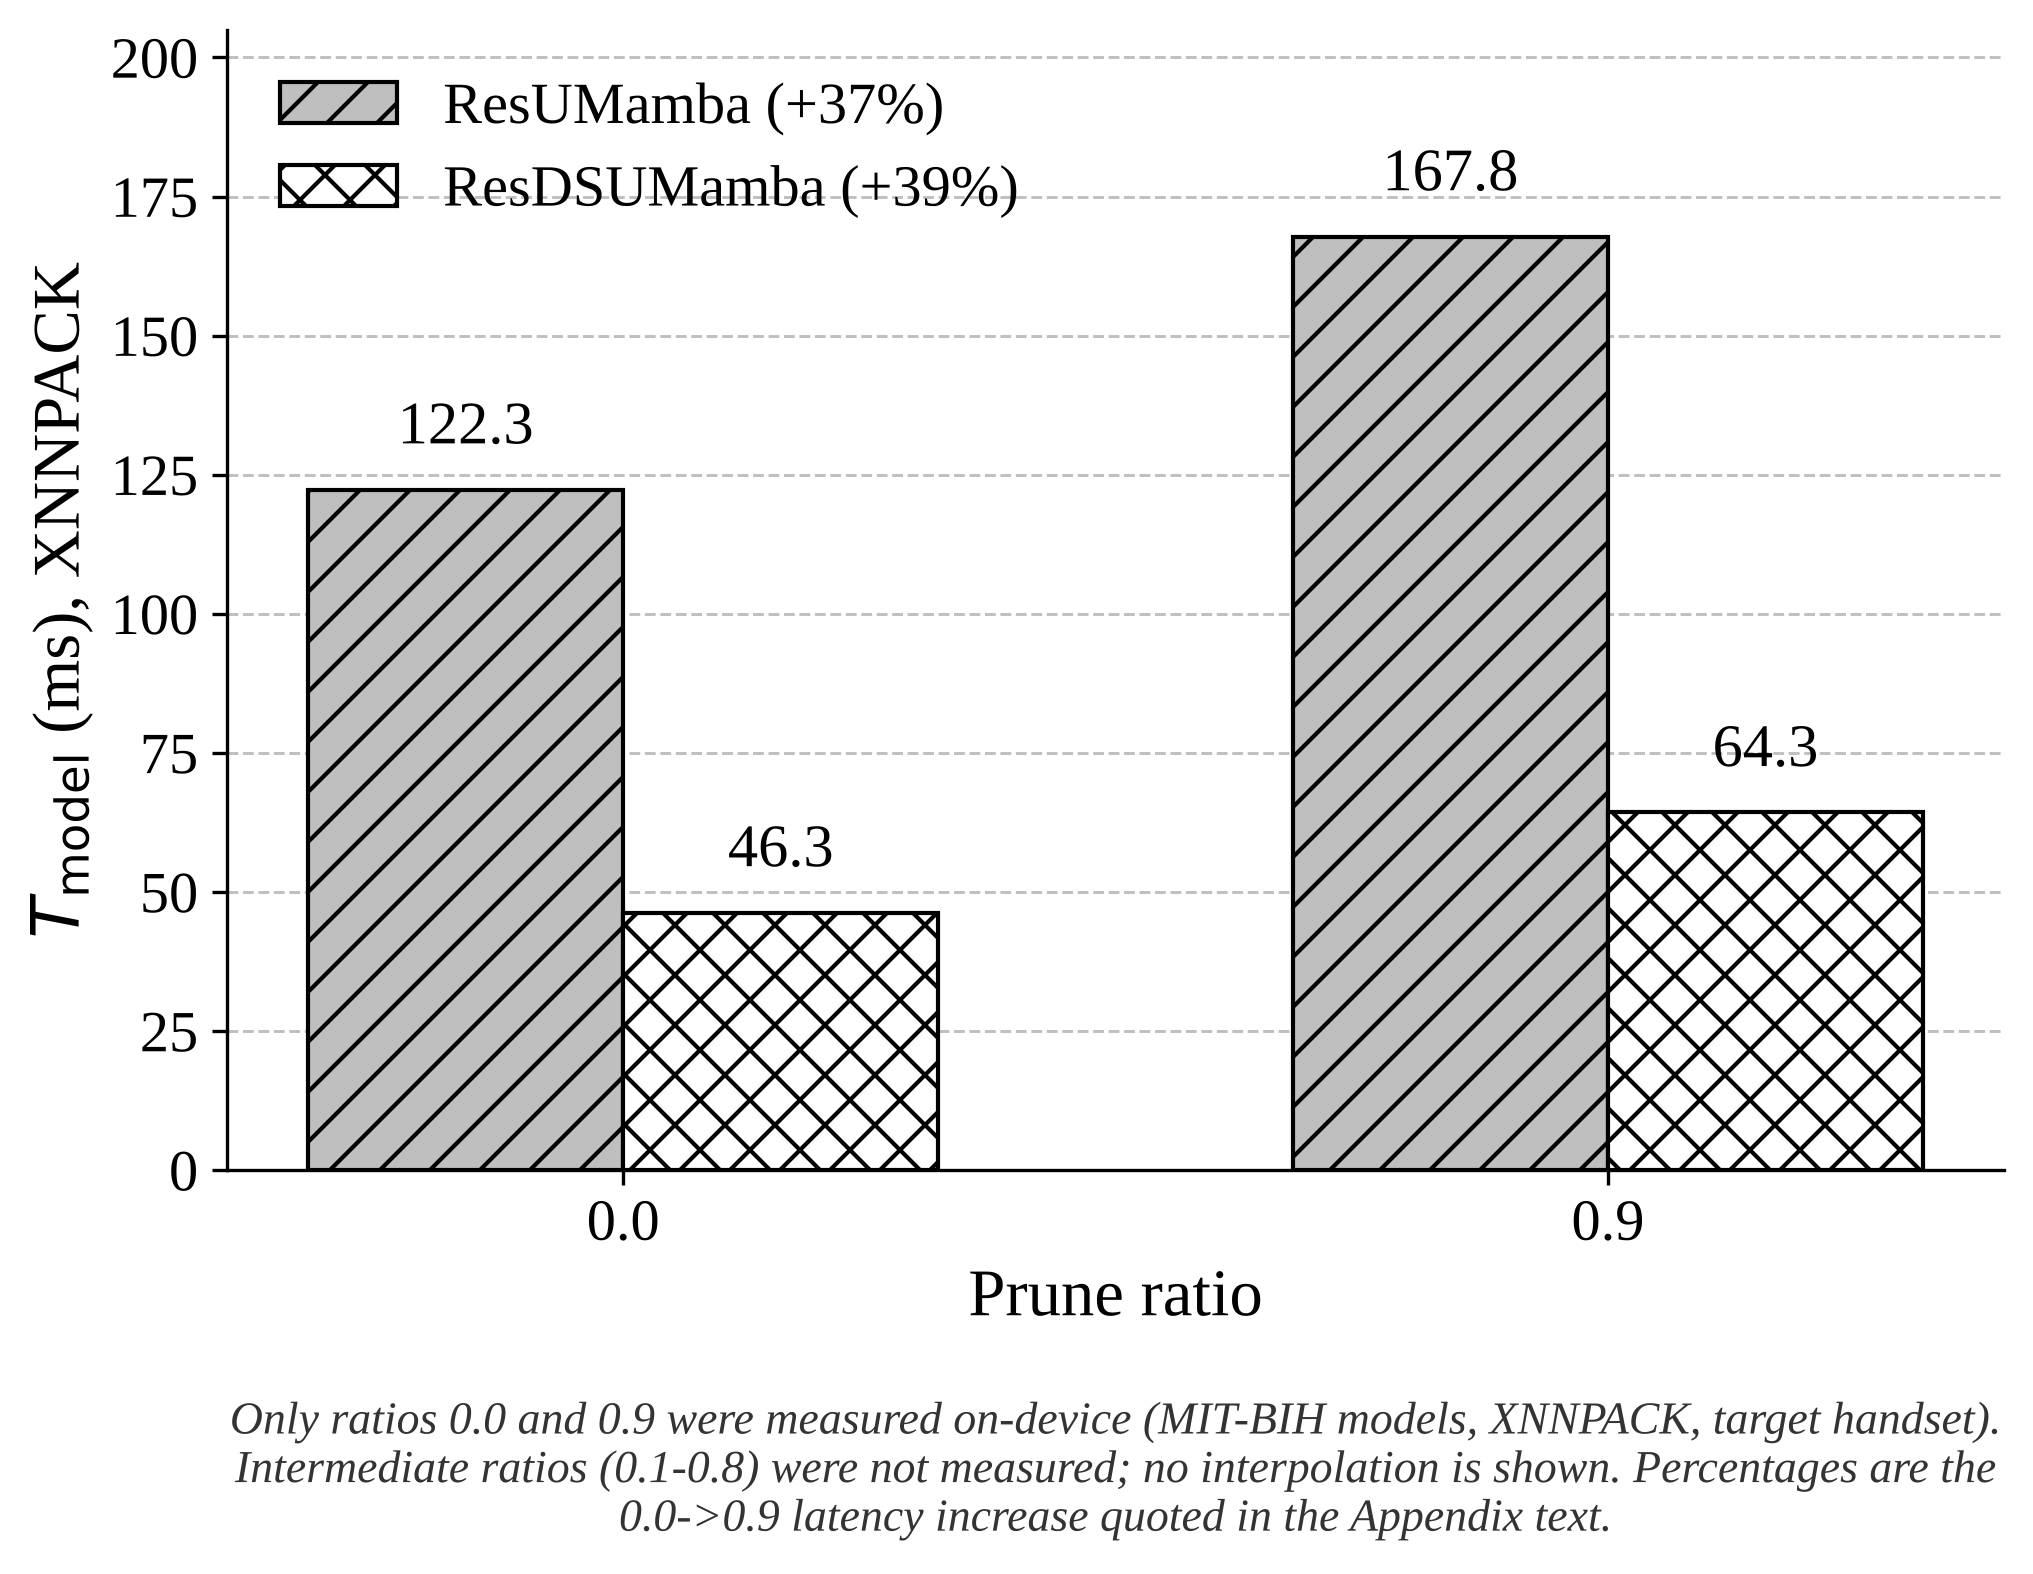
\includegraphics[width=0.7\textwidth]{figures/fig_pruning_latency.png}
  \caption[Mobile CPU latency versus prune ratio.]{Mobile CPU inference
  latency versus prune ratio on the target mobile handset using the
  XNNPACK delegate. Latency increases despite the increased prune ratio.}
  \label{fig:app_pruning_latency}
\end{figure}

Sparse representations can theoretically reduce storage, but this does
not imply a corresponding reduction in mobile CPU latency. As shown in
Fig.~\ref{fig:app_pruning_latency}, increasing the prune ratio did not
result in faster execution. On the target handset with the XNNPACK
delegate, the mean latency actually increased between ratios of $0.0$
and $0.9$: by $37\,\%$ for ResUMamba ($122.3$ to $167.8\,\mathrm{ms}$)
and by $39\,\%$ for ResDSUMamba ($46.3$ to $64.3\,\mathrm{ms}$).
The exported model files maintained the same size at both ratios,
indicating that the pruned weights were stored as zeros in dense
tensors, thus failing to reduce the actual operations executed on the
device.

Because structured pruning loses accuracy immediately and unstructured
pruning fails to provide a useful reduction in computation for the
target mobile deployment, pruning was deemed unsuitable. Consequently,
the depthwise separable convolution (DSConv) discussed in
Chapter~\ref{ch:optimization} was adopted to provide a structurally
reduced convolutional architecture with lower MACs and improved
suitability for mobile CPU execution.

\end{appendices}
